\section{aiman Implementation}

\subsection{System Architecture and Workflow}

The aiman tool is built using TypeScript and implements an intelligent command-line interface that helps users correct command-line operations. The system architecture follows a modular design that separates concerns between user interaction, command execution, AI processing, and data collection components.

\subsubsection{Core Components}

The CLI interface component (src/cli.ts) serves as the main entry point for user interaction, providing a colorful, user-friendly interface using chalk for visual feedback and readline for sophisticated input handling. This component manages the primary user experience and coordinates interactions with other system components.

Command execution functionality (src/commands.ts) handles the core operational requirements through Node.js child processes, capturing stdout, stderr, and exit codes to provide structured output for further processing. This component ensures reliable command execution while maintaining comprehensive logging of all system interactions.

Figure~\ref{fig:system_architecture} illustrates the high-level architecture of the aiman system, showing the interaction flow between user input, AI processing, and command execution.

\begin{figure}[h]
	\centering
	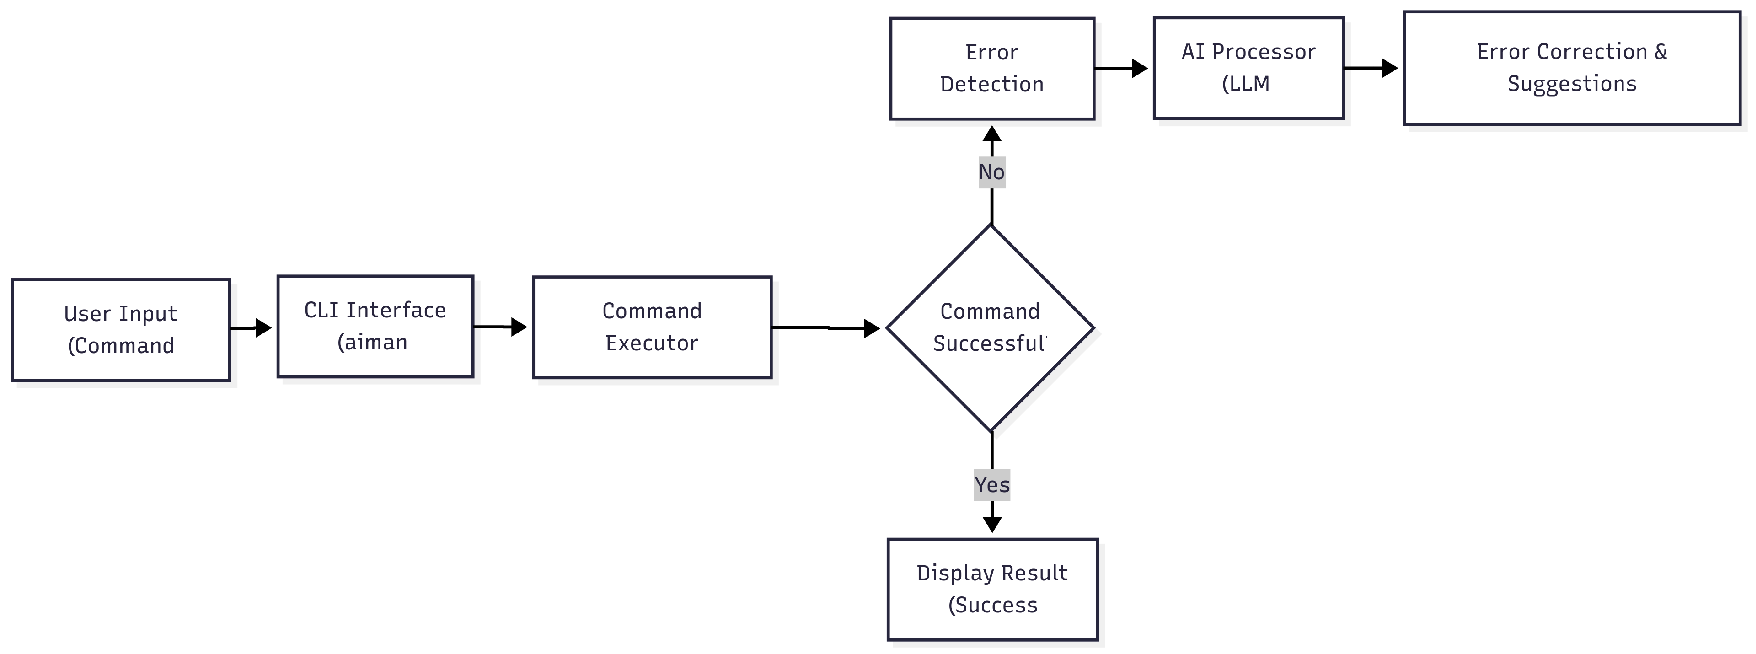
\includegraphics[width=0.9\textwidth]{assets/figures/system_architecture.pdf}
	\caption{aiman System Architecture Flow}
	\label{fig:system_architecture}
\end{figure}

Event handling (src/events.ts) manages the coordination between different system components, processing user input and orchestrating the interaction between command execution and AI assistance. This component handles error scenarios and AI help requests, ensuring smooth operation across different usage patterns.

\subsection{How AI Generates and Corrects Commands}

The AI correction system follows a structured workflow that analyzes failed commands and provides contextual assistance to users. This process begins when the system detects command failures and proceeds through a systematic analysis and correction pipeline.

\subsubsection{AI Processing Pipeline (src/llm.ts)}

When a command fails, the system captures comprehensive information including the original command, error output, and system environment information. This data collection ensures that AI assistance is provided with complete context for generating accurate corrections and explanations.

The AI help generation system provides two levels of assistance tailored to different user needs. Short help (getShortHelpForFailedCommand) provides concise assistance with essential correction information:

\begin{verbatim}
{
    error_explanation: string;
    corrected_command: string;
    explanation: string;
    tips: string;
}
\end{verbatim}

Detailed help (getHelpForFailedCommand) offers comprehensive assistance for users requiring more extensive guidance:

\begin{verbatim}
{
    error_explanation: string;
    corrected_command: string;
    arguments_explanation: string;
    best_practices: string;
}
\end{verbatim}

Response processing ensures system reliability through validation of JSON responses, calculation of API usage costs, and formatting of output with color coding for enhanced user experience. This processing layer maintains consistency and provides transparency about system resource usage.

\subsubsection{Environment Awareness}

The system (environments.ts) incorporates comprehensive environment detection capabilities that enhance the accuracy and relevance of AI assistance. These capabilities include detection of OS type and version, identification of terminal environment characteristics, provision of environment context to AI responses, and ensuring command compatibility across different system configurations. This environment awareness allows the AI to provide platform-specific recommendations and avoid suggesting commands that may not be available or behave differently across systems.

\subsection{Data Storage and Analytics}

The Store class (`evaluation/store.ts`) implements a comprehensive data management system designed for rigorous research data collection and analysis. The system employs UUID-based session tracking to maintain participant anonymity while enabling longitudinal analysis across multiple study sessions. Each participant session is uniquely identified and stored with complete metadata including timestamps, user demographics, and experimental conditions.

The data storage architecture uses JSON-based persistent storage with automatic file handling and directory creation. The system maintains both individual session data and aggregated multi-session datasets, automatically handling data format migrations and backwards compatibility. Performance metrics are collected at multiple granularities, including per-attempt timing data, command execution results, error classifications, and success indicators.

The Store class provides sophisticated session management capabilities, including condition order tracking for counterbalanced experimental designs, pre- and post-questionnaire data integration, and comprehensive test result aggregation. This enables researchers to analyze learning effects, fatigue patterns, and condition-specific performance variations across participants.

\subsection{Testing Framework Architecture}

The evaluation framework consists of four interconnected components that work together to provide systematic data collection and analysis capabilities:

\subsubsection{Test Execution Engine}

The \texttt{Test} class (\texttt{evaluation/test.ts}) executes individual command-line tasks. Each test instance contains a CLI challenge with multiple acceptable solutions, category classification (file navigation, file management, text processing, etc.), and optional pre-execution setup commands. The system validates commands using a two-tier assessment: exact string matching for known correct commands, followed by AI-based equivalence evaluation using the \texttt{compareCommandAndResults} function.

The test execution records timing data including user typing patterns, command execution duration, and total task completion time. Error handling categorizes failures into execution errors, incorrect commands, and skipped attempts. The system provides console feedback and logs all interactions for analysis.

\subsubsection{AI-Powered Command Assessment}

The framework uses AI validation through the \texttt{compareCommandAndResults} function in \texttt{llm.ts}. This function determines when alternative command formulations achieve equivalent results to expected solutions. The AI assessment evaluates both command syntax and execution output to recognize alternative approaches that exact-match systems would mark as incorrect.

The AI validator includes mechanisms to detect potentially dangerous commands (system deletion, security vulnerabilities) and provides explanations for assessment decisions. This approach handles complex commands with multiple valid formulations that would be difficult to enumerate manually.

\subsubsection{Orchestration and Condition Management}

The \texttt{user-tests.ts} module implements the study orchestration logic, managing participant flow through the complete experimental protocol. The system handles counterbalanced condition ordering (traditional-first vs. AI-first) with automatic alternation to prevent order effects. Command-line argument parsing enables flexible study configuration, including questionnaire skipping for rapid testing, test count limitations for pilot studies, and condition order forcing for debugging.

The orchestration system integrates pre- and post-study questionnaires, manages informed consent procedures, and provides comprehensive study information presentation. Progress tracking and session state management ensure reliable data collection even in the event of interruptions or technical difficulties.

\subsubsection{Interactive Command Processing}

The framework processes user commands through the \texttt{handleUserInput} function in \texttt{events.ts}, which provides different behavior based on experimental condition. In traditional mode, commands are executed with standard system feedback. In AI-assisted mode, failed commands trigger help generation through the \texttt{getShortHelpForFailedCommand} function, providing assistance without revealing solutions.

The command processing system includes error handling, output formatting, and timing instrumentation. Progress indicators provide user feedback during AI processing, and logging captures user interaction patterns and system performance.

This framework enables comparison of traditional and AI-assisted CLI interfaces while maintaining experimental controls and data collection for usability research.

\subsection{Error Handling and User Assistance}

The system implements error handling that provides context-aware error messages to help users understand command failures. The mechanism suggests corrections based on common patterns and provides guidance for future usage. The error handling approach addresses immediate problems while providing educational information.

This implementation executes commands and provides error correction and assistance. The modular architecture separates concerns while the data collection capabilities support experimental evaluation.

\subsubsection{Cost Management and Optimization}

The system implements transparent cost tracking through calculateCost in utils.ts, which tracks prompt and completion tokens separately, uses different rates for different token types, and provides transparency by showing costs to users. This cost management approach ensures responsible resource usage while maintaining user awareness of system expenses.

\subsubsection{Extensibility}

The system demonstrates strong modular design principles through its TypeScript architecture with separate components for CLI, commands, events, LLM processing, and evaluation functions. Additionally, the system provides configurable test scenarios through JSON configuration files, extensible metrics collection with customizable data storage, and command-line argument parsing for different operational modes. These design choices highlight the maintainability of the aiman implementation, demonstrating how it separates concerns between command execution, AI processing, and data collection to provide researchers with a flexible tool for conducting CLI usability experiments.

\section{Comparative Testing Framework}

This experiment compares different command-line interfaces (CLI) in terms of usability and error correction effectiveness. The study evaluates two variations to capture the effects of AI assistance:

\begin{enumerate}
	\item \textbf{Traditional CLI (Control):} The native Linux/macOS terminal without AI assistance.
	\item \textbf{aiman (AI Assistance on Error):} The AI provides suggestions only when the user enters an invalid or failing command.
\end{enumerate}

\subsection{Primary Objectives (Dependent Variables)}

The primary objective focuses on measuring efficiency through how effectively users complete CLI tasks, including metrics such as task completion time, number of errors, and retry attempts. This efficiency measurement provides quantitative evidence of the practical benefits offered by AI assistance in command-line environments.

Command-line interfaces (CLIs) offer powerful capabilities, but their usability is often limited by a steep learning curve, requiring memorization of syntax, flags, and command structures. Prior research highlights how users—especially novices—struggle with syntactic errors, conceptual mismatches, and the indirectness of interaction \cite{margono1987}. To mitigate these challenges, intelligent agents that learn from user behavior and suggest or correct commands have been proposed. For example, Hirsh \& Davison (1997) embedded a predictive assistant in tcsh that suggested next commands based on history, achieving up to 67\% prediction accuracy \cite{hirsh1997}. Their system demonstrated the feasibility of integrating machine learning into interactive CLI environments to support user intent.

Building on this foundation of predictive and corrective CLI support, our work evaluates whether real-time AI assistance can improve usability in error-prone scenarios. Unlike Hirsh \& Davison, who focused on prediction accuracy, we focus on user outcomes—task success, correction time, and satisfaction—aligning with calls in their paper for more meaningful performance measures. Our task set is grounded in empirical studies of real-world shell usage: Gharehyazie et al. (2016) analyzed over 1 million shell commands across 263 users and found that cd, ls, grep, find, and other file-management commands are central to everyday shell usage \cite{gharehyazie2016}. Additionally, we incorporate the novice-focused curriculum structure outlined by Wilson (2016), in which Software Carpentry emphasizes a canonical progression through Unix shell, Git version control, and Python/R scripting as core competencies \cite{wilson2016}.

\subsection{Participant Selection and Recruitment}

The study targets experienced software engineers with 3–10 years of professional experience as the primary participant group. This population is selected because they are proficient with computers and likely familiar with CLI basics, which helps focus the study on efficiency gains and subtle improvements rather than basic learning effects.

Participant selection follows specific inclusion and exclusion criteria to ensure appropriate study population characteristics. Inclusion criteria encompass professional software development experience (3+ years), regular computer usage in professional contexts, basic familiarity with terminal/command-line environments, and willingness to participate in controlled testing sessions. Exclusion criteria eliminate expert-level CLI masters (to avoid ceiling effects) and complete CLI novices (to ensure task feasibility).

Within-subjects designs typically require fewer participants than between-subjects designs because each person serves as their own control, reducing individual variation. Based on effect size estimates from similar HCI studies and practical feasibility constraints, we target 6-10 participants to achieve adequate statistical power for detecting meaningful differences in task completion time, success rates, and number of attempts.

Participants are recruited through professional networks, software development communities, and academic contacts. Prior to the experiment, each participant completes a pre-survey detailing their background (years of experience, self-rated CLI proficiency, usage frequency, etc.) to contextualize the results and ensure they meet inclusion criteria.

\subsection{Apparatus and Environment}

The experiment was conducted on a Linux virtual machine (VM) in a Dockerized environment accessed via SSH. This setup provides a standardized CLI environment for all participants, ensuring consistency across testing sessions and eliminating variations in local system configurations.

The baseline interface utilizes the native terminal (e.g. Bash or Zsh shell on a typical Terminal app), providing no special assistance beyond standard shell features. In contrast, the aiman tool integrates a generative AI assistant into the terminal, which can detect command errors or incomplete commands and suggest corrections or completions in real-time. Key features of aiman include syntax correction and suggestions when a command fails or is likely incorrect, and enhanced help or examples when the user is unsure of a command.

An interactive testing harness (included in the aiman codebase) presents tasks and records data systematically. This harness presents task descriptions to users in the terminal, accepts their command input, and automatically logs outcomes. In traditional mode, it records the commands entered and determines task success by monitoring command exit codes (0 for success, non-zero for failure) and validating expected output patterns. In aiman mode, it also logs AI suggestions made and whether the user accepted or ignored them.

All sessions are conducted within the same Docker container environment to ensure identical system configurations. Participants connect to the VM via SSH, providing a consistent terminal experience regardless of their local machine. Internet access is available for tasks requiring network operations, and comprehensive logging captures all command inputs and outputs through the built-in JSON-based data collection system. Before starting, each system is reset to a clean state (e.g. clearing any command history that could give hints) and loaded with any files or directories needed for the tasks (for example, sample directories to search in, or specific files to manipulate).

\section{Data Collection \& Evaluation Metrics}

Multiple quantitative metrics are collected to evaluate performance on each task and across conditions. Table \ref{tab:metrics} summarizes the key metrics and their definitions:

\begin{table}[h]
	\centering
	\small
	\begin{tabular}{|p{2.5cm}|p{4cm}|p{4.5cm}|}
		\hline
		\textbf{Metric} & \textbf{Description} & \textbf{Collection Method} \\
		\hline
		Task Completion Time & Time from task presentation to successful completion (seconds) & Automatic timestamps by testing harness \\
		\hline
		Success Rate & Binary task completion success (success/failure) & Derived from command logs and exit codes \\
		\hline
		Number of Attempts & Total command attempts before task completion & Count from command log per task \\
		\hline
		Error Rate & Percentage of tasks with execution errors, incorrect commands, or skips & Calculated from error classifications in logs \\
		\hline
		Ease of Use Rating & Comparative assessment of interface usability (5-point scale) & Post-experiment Likert questionnaire (1=Traditional easier, 5=AI easier) \\
		\hline
		Confidence Rating & Comparative assessment of user confidence (5-point scale) & Post-experiment Likert questionnaire (1=Traditional more confident, 5=AI more confident) \\
		\hline
		Frustration Rating & Comparative assessment of interface frustration (5-point scale) & Post-experiment Likert questionnaire (1=Traditional more frustrating, 5=AI more frustrating) \\
		\hline
	\end{tabular}
	\caption{Key Metrics for Evaluation}
	\label{tab:metrics}
\end{table}

All these metrics align with standard usability measures: efficiency (time and attempts), effectiveness (success rates and error patterns), and satisfaction (ease of use, confidence, and frustration ratings). Data is collected through automated logging within the interactive testing harness, which captures all command inputs, outputs, timing information, and AI interactions in JSON format.

\section{Data Analysis and Visualization Tools}

The experimental data collected through the aiman testing framework is processed using a custom analysis pipeline to extract insights from CLI usability experiments. This section outlines the analysis approach and tools used to process and visualize the experimental results.

\subsection{Analysis Pipeline Overview}

The data analysis follows a two-stage pipeline that transforms raw experimental data into statistical summaries and visualizations. The first stage focuses on statistical analysis, where raw JSON data from participant sessions is processed to calculate key performance metrics, error patterns, and user satisfaction measures. The analysis tool handles data validation, calculates derived metrics, and generates statistical summaries across multiple dimensions including overall performance, task categories, participant demographics, and CLI proficiency correlations.

The second stage involves visualization generation, where statistical results are converted into charts and graphs using a visualization pipeline. This includes performance comparison charts, error analysis visualizations, user satisfaction plots, and demographic distributions.

\subsection{Analysis Capabilities}

The analysis pipeline covers experimental data across several analytical dimensions. Performance analysis encompasses success rates, completion times, and attempt counts for both traditional and AI-assisted conditions, task category breakdowns (file navigation, text processing, system administration, etc.), and individual test performance comparisons.

Error pattern analysis provides classification and quantification of error types across interface conditions, user-generated error analysis (excluding prefilled incorrect commands), and common failure pattern identification with AI correction effectiveness assessment.

User experience analysis processes Likert scale responses for ease of use, confidence, and frustration metrics, conducts preference rating analysis with statistical summaries, and performs correlation analysis between objective performance and subjective satisfaction.

Demographic and proficiency analysis examines performance variation across participant characteristics, CLI proficiency correlation with task success rates, and condition order effect analysis for experimental validity.

\subsection{Data Processing and Quality Assurance}

The analysis tools include comprehensive data processing with quality assurance measures. Data integrity validation ensures completeness and structure, with appropriate handling of missing or incomplete entries. Statistical robustness is maintained through proper handling of edge cases, small sample sizes, and missing data points with transparent reporting of limitations. Reproducibility is ensured through consistent processing algorithms with deterministic output generation for replication of analysis results.

\subsection{Output Generation}

The analysis pipeline produces multiple output formats to support different research and presentation needs. Statistical reports provide text-based summaries with key findings, performance metrics, and statistical indicators. Structured data exports in JSON and CSV formats enable integration with external statistical software and further analysis. Visualizations include charts for performance comparisons, error analysis plots, user satisfaction graphics, and demographic distributions.

This analysis infrastructure processes experimental data while maintaining flexibility to adapt to different research questions and presentation requirements.
